\documentclass[10pt,a4paper]{article}
\usepackage{amsmath}
\usepackage{amssymb}
\usepackage{graphicx}
\usepackage{color}
\usepackage{fancyhdr}
\usepackage{fancyvrb}
\usepackage[margin=3.5cm]{geometry}
\usepackage{framed}
\usepackage{enumerate}
\usepackage{textcomp}
\def\ket#1{\left|#1\right\rangle}
\def\bra#1{\left\langle#1\right|}
\def\braket#1{\left\langle#1\right\rangle}

\definecolor{linkcol}{rgb}{0.0, 0.0, 0.5}
\usepackage[colorlinks=true,urlcolor=linkcol,citecolor=black,linkcolor=linkcol]{hyperref}

\renewcommand\thesection{4.\arabic{section}}
\renewcommand\thesubsection{\thesection.\arabic{subsection}}

\fancyhf{}
\lhead{\tiny Y.~D.~Chong (2016)}
\rhead{\scriptsize MH2801: Complex Methods for the Sciences}
\lfoot{}
\rfoot{\thepage}
\pagestyle{fancy}

\makeatletter
\def\PY@reset{\let\PY@it=\relax \let\PY@bf=\relax%
    \let\PY@ul=\relax \let\PY@tc=\relax%
    \let\PY@bc=\relax \let\PY@ff=\relax}
\def\PY@tok#1{\csname PY@tok@#1\endcsname}
\def\PY@toks#1+{\ifx\relax#1\empty\else%
    \PY@tok{#1}\expandafter\PY@toks\fi}
\def\PY@do#1{\PY@bc{\PY@tc{\PY@ul
\def\PYZdl{\char`\$}
\def\PYZhy{\char`\-}
\def\PYZsq{\char`\'}
\def\PYZdq{\char`\"}
\def\PYZti{\char`\~}

\begin{document}
\setcounter{page}{27}
\noindent
\underline{\textbf{\LARGE 4. Complex Oscillations}}
\vskip 0.1in

The most common use of complex numbers in physics is for analyzing
oscillations and waves. We will illustrate this with a simple but
crucially important model, the \textbf{damped harmonic oscillator}.

\section{The harmonic oscillator equation}
\label{the-harmonic-oscillator-equation}

The damped harmonic oscillator describes a mechanical system consisting
of a particle of mass $m$, subject to a spring force and a damping
force:

\begin{figure}[h]
  \centering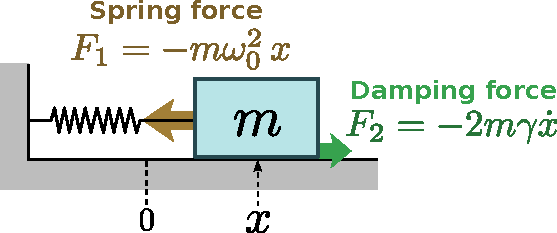
\includegraphics[width=0.45\textwidth]{oscillator}
\end{figure}
\noindent
The particle can move along one dimension, and we let $x(t)$ denote
its displacement from the origin. The damping coefficient is $2m
\gamma$, and the spring constant is $k = m\omega_0^2$. The parameters
$m$, $\gamma$, and $\omega_0$ are all positive real numbers. (The
quantity $\omega_0$ is called the ``natural frequency of
oscillation'', because in the absence of the damping force this system
would act as a simple harmonic oscillator with frequency $\omega_0$.)

The motion of the particle is described by Newton's second law:
\begin{equation}
  m \frac{d^2 x}{dt^2} = F(x,t) = - 2m\gamma \frac{dx}{dt} - m\omega_0^2 x(t).
\end{equation}
Dividing by the common factor of $m$, and bringing everything to one
side, gives
\begin{equation}
  \frac{d^2 x}{dt^2} + 2\gamma \frac{dx}{dt} + \omega_0^2 x(t) = 0.
\end{equation}
We call this ordinary differential equation the \textbf{damped
  harmonic oscillator equation}. Since it's a second-order ordinary
differential equation (ODE), the general solution must contain two
independent parameters. If we state the initial displacement and
velocity, $x(0)$ and $\dot{x}(0)$, there is a unique specific
solution.

\begin{framed}
\noindent
\underline{\textbf{Note}}
\vskip 0.1in \noindent
Sometimes, we write the damped harmonic oscillator equation a bit
differently:
\begin{equation}
\left[\frac{d^2}{dt^2} + 2\gamma \frac{d}{dt} + \omega_0^2 \right]\, x(t) = 0.
\end{equation}The
quantity in the square brackets is regarded as an operator acting on
$x(t)$. This operator consists of the sum of three terms: a
second-derivative operator, a constant times a first derivative, and
multiplication by a constant.
\end{framed}

We are interested in solving for $x(t)$.  For the simple (undamped)
harmonic oscillator, which is the case where $\gamma = 0$, we know
what the general solution looks like:
\begin{equation}
  x(t) = x_0 \cos(\omega_0 t + \phi).
\end{equation}
The particle oscillates around the equilibrium position, $x = 0$,
because the spring force keeps pushing it towards the origin and its
momentum causes it to ``overshoot''.  For the damped harmonic
oscillator ($\gamma > 0$), however, the damping force causes the
particle to lose energy during its motion, so that as $t \rightarrow
\infty$, both $x$ and $\dot{x}$ go to zero.  A typical solution is
shown in the following figure:

\begin{figure}[h]
  \centering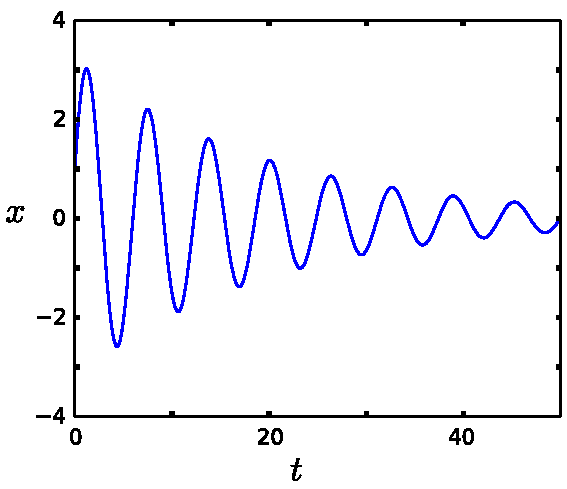
\includegraphics[width=0.4\textwidth]{damped_oscillator_motion}
\end{figure}

\section{Complex solution}
\label{complex-solution}

The variable $x(t)$ stands for the displacement of a particle, which
is a real quantity. But in order to solve the damped harmonic
oscillator equation, it's useful if we generalize $x(t)$ to complex
values. In other words, let's treat the harmonic oscillator equation
as a \emph{complex} ODE:
\begin{equation}
\frac{d^2 z}{dt^2} + 2\gamma \frac{dz}{dt} + \omega_0^2 z(t) = 0, \quad z(t) \in \mathbb{C}.
\label{zode}
\end{equation}
The parameter-counting rule that we discussed for real ODEs can also
be applied to complex ODEs, except that we use complex parameters in
place of real parameters. In this case, the complex damped harmonic
oscillator equation is a second-order ODE, so its general solution
should contain two independent \emph{complex} parameters.

Once we have that general solution, we can do one of two things: (i)
plug in a complete set of (real) boundary conditions, which will give
a real specific solution, or (ii) take the real part of the complex
general solution, which will give the general solution to the real
differential equation. We will discuss these two approaches later; for
the moment, let's focus on finding the solution to the complex ODE.

To find the complex solution, first note that the equation is linear.
This means that if we have two solutions $z_1(t)$ and $z_2(t)$, then
any combination
\begin{equation}
  \alpha \, z_1(t) + \beta \,z_2(t),\quad \mathrm{where}\;\; \alpha, \beta \in \mathbb{C}
\end{equation}
is also a solution. Therefore, a good strategy is to find several
specific solutions, and then combine them linearly to form a more
general solution. We simply make a guess (or an \textbf{ansatz}) for a
specific solution:
\begin{equation}
  z(t) = e^{-i\omega t}, \label{zansatz}
\end{equation}
where $\omega$ is a constant to be determined (it could be
complex). The first and second derivatives of Eq.~(\ref{zansatz}) are:
\begin{align}
  \frac{dz}{dt} &= -i\omega\, e^{-i\omega t} \\
  \frac{d^2z}{dt^2} &= -\omega^2\, e^{-i\omega t}
\end{align}
Substituting these into the differential equation (\ref{zode}) gives:
\begin{equation}
  \left[-\omega^2 - 2i\gamma \omega + \omega_0^2 \right] e^{-i\omega t} = 0.
\end{equation}
This equation can be satisfied for all $t$ if the complex quadratic on
the left side is zero:
\begin{equation}
  -\omega^2 - 2i\gamma \omega + \omega_0^2 = 0.
\end{equation}
In other words, we need values of $\omega$ which solve this quadratic
equation. The solutions can be obtained from the quadratic formula:
\begin{equation}
  \omega = -i\gamma \pm \sqrt{\omega_0^2 - \gamma^2}.
\end{equation}
Hence, we arrive at solutions which are oscillations with
\emph{complex} frequencies:
\begin{equation}
z(t) = \exp\left(-i\omega_\pm t\right), \;\;\mathrm{where}\;\; \omega_\pm = -i\gamma \pm \sqrt{\omega_0^2 - \gamma^2}.
\end{equation}
For each value of $\gamma$ and $\omega_0$, there are two possible
frequencies, $\omega_+$ and $\omega_-$. For either choice of complex
frequency, the above expression for $z(t)$ gives a valid specific
solution for the complex damped harmonic oscillator equation.

\subsection{Complex frequencies}
\label{complex-frequencies}

What does it mean to have an oscillation with a complex frequency? If
we write the real and imaginary parts of the frequency as $\omega =
\omega_R + i \omega_I$, then
\begin{equation}
  z(t) = e^{-i\omega t} = e^{\omega_I t} \; e^{-i\omega_R t}.
\end{equation}
If both $\omega_R$ and $\omega_I$ are non-zero, this describes a
spiral trajectory in the complex plane, whose magnitude is either
increasing or decreasing with time, depending on the sign of
$\omega_O$. This is because we can write
\begin{equation}
  z(t) = e^{\omega_I t} \; e^{-i\omega_R t} = R(t)\, e^{i\theta(t)}, \;\;\mathrm{where}\;\;R(t) = e^{\omega_I t}, \; \theta(t) = -\omega_R t.
\end{equation}
We therefore conclude that the real part of $\omega$ determines the
(angular) frequency of oscillation, whereas the imaginary part
determines whether the oscillation amplitude is either growing with
time (amplification) or shrinking with time (damping). A positive
imaginary part implies amplification, and a negative imaginary part
implies damping, while zero imaginary part (i.e., a real frequency)
implies constant-amplitude oscillation.

Now let's look at the damped harmonic oscillator's complex
frequencies:
\begin{equation}
  \omega_\pm = -i\gamma \pm \sqrt{\omega_0^2 - \gamma^2}.
\end{equation}
These depend on two real parameters: $\gamma$ and $\omega_0$. In the
plot below, you can see how the position of $\omega_\pm$ in the
complex plane depends on the values of these parameters.

\begin{figure}[h]
  \centering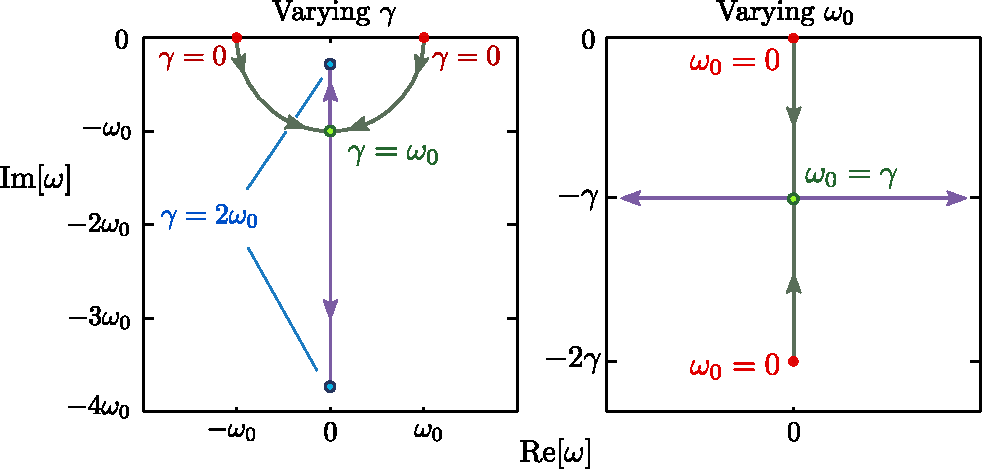
\includegraphics[width=0.75\textwidth]{oscillator_frequencies}
\end{figure}

\pagebreak
\noindent
In particular, note the following features:
\begin{itemize}
\item
  For $\gamma = 0$ (zero damping), the two frequencies are both real,
  and take the values $\pm \omega_0$. This corresponds to undamped (or
  ``simple'') harmonic oscillation at the oscillator's natural
  frequency.
\item
  If we increase $\gamma$ from zero with $\omega_0$ fixed, both
  $\omega_+$ and $\omega_-$ move downwards in the complex plane,
  along a circular arc. Because the imaginary part of the frequencies
  are negative, this implies damped oscillation.

\item
  At $\gamma = \omega_0$, the frequencies meet along the imaginary
  axis.

\item
  For $\gamma > \omega_0$, the two frequencies move apart along the
  imaginary axis. Purely imaginary frequencies correspond to a
  trajectory that simply decays without oscillating.
\end{itemize}

\section{General solution for the damped harmonic oscillator}
\label{general-solution}

For now, suppose $\omega_0 \ne \gamma$. In the previous section, we
found two classes of specific solutions, with complex frequencies
$\omega_+$ and $\omega_-$:
\begin{equation}
  z_+(t) = e^{-i\omega_+ t} \;\;\mathrm{and}\;\;
  z_-(t) = e^{-i\omega_- t}, \;\;\mathrm{where}\;\;\;
  \omega_\pm = -i\gamma \pm \sqrt{\omega_0^2 - \gamma^2}.
\end{equation}
We can write down a more general solution consisting of a linear
superposition of these specific solutions:
\begin{align}
  z(t) &= \psi_+ e^{-i\omega_+ t} + \psi_- e^{-i\omega_- t} \\
  &= \psi_+ \, \exp\left[\left(-\gamma  - i \sqrt{\omega_0^2 - \gamma^2}\right)t\right] \; +\; \psi_- \, \exp\left[\left(-\gamma +i\sqrt{\omega_0^2 - \gamma^2}\right)t\right].
\end{align}
This contains two undetermined complex parameters, $\psi_+$ and
$\psi_-$. These are \emph{independent} parameters since they are the
coefficients that multiply different functions (the functions are
different because $\omega_0 \ne \gamma$ implies that $\omega_+ \ne
\omega_-$). Hence, the above equation for $z(t)$ is a general solution
for the complex damped harmonic oscillator equation.

To obtain the general solution to the \emph{real} damped harmonic
oscillator equation, we have to take the real part of the complex
solution. The result can be further simplified depending on whether
$\omega_0^2 - \gamma^2$ is positive or negative.  This leads to what
are called \textbf{under-damped solutions} and \textbf{over-damped
  solutions}, to be discussed in the following subsections.

What about if $\omega_0 = \gamma$? In this instance, $\omega_+ =
\omega_-$, which means that $\psi_+$ and $\psi_-$ aren't independent
parameters. Therefore, the above equation for $z(t)$ isn't a valid
general solution in this particular case!  Instead, the general
solution is something called a \textbf{critically-damped solution},
which we will \hyperref[critical-damping]{discuss in Section
  \ref{critical-damping}}.

\subsection{Under-damped motion}
\label{under-damped-motion}

For $\omega_0 > \gamma$, let us define, for convenience,
\begin{equation}
  \Omega = \sqrt{\omega_0^2 - \gamma^2}.
\end{equation}
Then we can simplify the real solution as follows:

\begin{align}
  x(t) &= \mathrm{Re}\left[z(t)\right] \\
  &= e^{-\gamma t} \; \mathrm{Re}\left[\psi_+ \, e^{-i \Omega t} \,+\, \psi_- \, e^{i\Omega t}\right] \\
  &= e^{-\gamma t} \left[ A\cos\left(\Omega t\right) + B \sin\left(\Omega t\right)\right], \;\;\mathrm{where}\;\; A, B \in \mathbb{R}
\end{align}
With a bit of algebra, we can show that
\begin{equation}
  A = \mathrm{Re}\left[\psi_+ + \psi_-\right],
  \quad B = \mathrm{Im}\left[\psi_+ - \psi_-\right].
\end{equation}
The coefficients $A$ and $B$ act as two independent \emph{real}
parameters, so this is a valid general solution for the real damped
harmonic oscillator equation. Using the trigonometric formulas, the
solution can be equivalently written as
\begin{equation}
x(t) = C e^{-\gamma t} \cos\left[\Omega t + \Phi\right],
\end{equation}
with the parameters $C = \sqrt{A^2 + B^2}$ and $\Phi = -
\tan^{-1}\left[B/A\right]$.

Either way, this is called an \textbf{under-damped solution}. A
typical graph is shown below:

\begin{figure}[h]
  \centering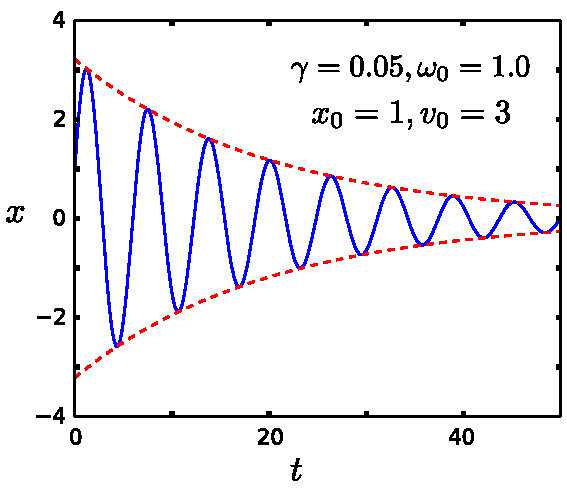
\includegraphics[width=0.5\textwidth]{underdamped}
\end{figure}

\noindent
The particle undergoes oscillation, but the amplitude of oscillation
decreases with time. The decrease in the amplitude can be visualized
using a smooth ``envelope'' given by $\pm C e^{-\gamma t}$, which is
drawn with dashes in the figure. Inside this envelope, the trajectory
oscillates with frequency $\Omega = \sqrt{\omega_0^2 - \gamma^2}$,
which is slightly less than the natural frequency of oscillation
$\omega_0$.

\subsection{Over-damped motion}\label{over-damped-motion}

For $\omega_0 < \gamma$, the square root term becomes imaginary. It is
convenient to define
\begin{equation}
  \Gamma = \sqrt{\gamma^2 - \omega_0^2} \quad \Rightarrow \quad \sqrt{\omega_0^2 - \gamma^2} = i \Gamma.
\end{equation}
Then the real solution simplifies in a different way:
\begin{align}
  x(t) &= \mathrm{Re}\left[z(t)\right] \\
  &= \mathrm{Re}\left[\psi_+ e^{\left(-\gamma  + \Gamma\right)t} + \psi_- e^{\left(-\gamma - \Gamma\right)t} \right] \\
  &= C_+ e^{-(\gamma - \Gamma) t} + C_- e^{-(\gamma + \Gamma) t},
\end{align}
where
\begin{equation}
  C_\pm = \mathrm{Re}[\psi_\pm].
\end{equation}
This is called an \textbf{over-damped} solution. The solution consists
of two terms, both exponentially decaying in time, with
$(\gamma-\Gamma)$ and $(\gamma + \Gamma)$ serving as the decay
rates. Note that both decay rates are positive real numbers, because
$\Gamma < \gamma$ from the definition of $\Gamma$. Also, note that the
first decay rate $(\gamma - \Gamma)$ is a \emph{decreasing} function
of $\gamma$, whereas the second decay rate $(\gamma + \Gamma)$ is an
\emph{increasing} function of $\gamma$.
    
The larger decay rate, $(\gamma + \Gamma)$, is associated with a
faster-decaying exponential. Therefore, at long times the second term
becomes negligible compared to the first term. Then the solution
approaches the limit
\begin{equation}
  x(t) \approx C_+ e^{-(\gamma - \Gamma) t} \qquad (\mathrm{large}\;\;t).
\end{equation}
This limiting curve is shown as a red dash in the figure below.

\begin{figure}[h]
  \centering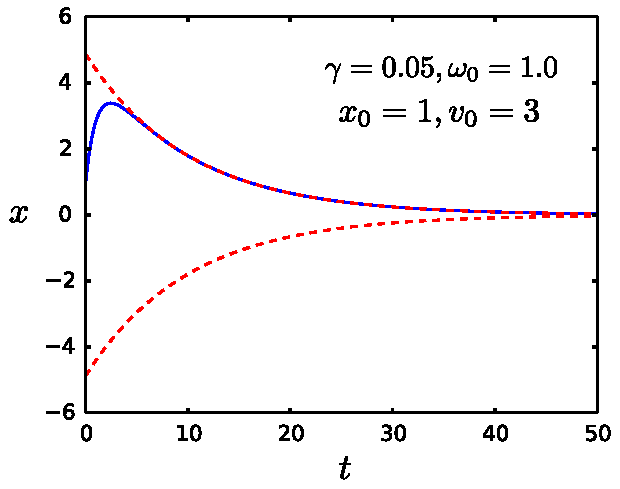
\includegraphics[width=0.5\textwidth]{overdamped}
\end{figure}

\noindent
This has an interesting implication: \emph{the stronger the damping,
  the slower the effective decay rate at long times}. Why does this
happen? In the over-damped regime, the motion of the oscillator is
dominated by the damping force rather than the spring force; as the
oscillator tries to return to its equilibrium position $x = 0$, the
damping acts against this motion. Hence, the stronger the damping, the
slower the decay to equilibrium.

This contrasts sharply with the
\hyperref[under-damped-motion]{previously-discussed under-damped
  regime}, where the spring force dominates the damping force.  There,
stronger damping speeds up the decay to equilibrium, by causing the
kinetic energy of the oscillation to be dissipated more rapidly.

\subsection{Critical damping}
\label{critical-damping}

\textbf{Critical damping} occurs when $\omega_0 = \gamma$. Under this
special condition, \hyperref[general-solution]{the solution we
  previously derived} reduces to
\begin{equation}
  z(t) = \left(\psi_+ + \psi_-\right) e^{-\gamma t}.
\end{equation}
This has only \emph{one} independent complex parameter, i.e.~the
parameter $(\psi_+ + \psi_-)$. Therefore, it cannot be a general
solution for the complex damped harmonic oscillator equation, which is
still a second-order ODE.

We will not go into detail here regarding the procedure for finding
the general solution for the critically-damped oscillator, leaving it
as an exercise for the interested reader.  Basically, we can Taylor
expand the solution on either side of the critical point, and then
show that there is a solution of the form
\begin{equation}
  z(t) = \left(A + B t\right)\, e^{-\gamma t},
\end{equation}
which contains the desired two independent parameters.

The critically-damped solution contains an exponential decay constant
of $\gamma$, which is the same as the decay constant for the
\hyperref[under-damped-motion]{envelope function in the under-damped
  regime}, and smaller than the (long-time) decay constants in the
\hyperref[over-damped-motion]{over-damped regime}. Hence, we can
regard the critically-damped solution as the \emph{fastest-decaying
  non-oscillatory solution}.

This feature of critical damping is employed in many engineering
contexts, the most familiar being automatic door closers. If the
damping is too weak or the spring force is too strong (under-damped),
the door will tend to slam shut, whereas if the damping is too strong
or the spring force is too weak (under-damping), the door will take
unnecessarily long to close. Hence, door closers need to be tuned to a
``sweet spot'' that corresponds to the critical damping point.

\section{Stating the solution in terms of initial conditions}
\label{initial-conditions}

The \hyperref[general-solution]{general solution for the complex
  damped harmonic oscillator equation} contains two undetermined
parameters which are the complex amplitudes of the ``clockwise'' and
``counterclockwise'' complex oscillations:
\begin{equation}
z(t) = \psi_+ e^{-i\omega_+ t} + \psi_- e^{-i\omega_- t}, \quad\mathrm{where} \;\; \omega_\pm =  -i\gamma  \pm \sqrt{\omega_0^2 - \gamma^2}.
\end{equation}
However, mechanics problems are often expressed in terms of an
\textbf{initial-value problem}, which expresses the state of the
system at some initial time $t = 0$. Suppose we are given $z(0) \equiv
x_0$ and $\dot{z}(0) \equiv v_0$; then what is $z(t)$ in terms of
$x_0$ and $v_0$?

We can solve the initial-value problem by finding $z(0)$ and
$\dot{z}(0)$ in terms of the above general solution for $z(t)$. The
results are
\begin{align}
  z(0) &= \quad \psi_+ + \psi_- \qquad\quad = x_0& \\
  \dot{z}(0) &= -i\omega_+ \psi_+ - i \omega_- \psi_- = v_0.&
\end{align}
These two equations can be combined into a $2\times2$ matrix equation:
\begin{equation}
  \begin{bmatrix}1 & 1 \\ -i\omega_+ & -i\omega_-\end{bmatrix} \begin{bmatrix}\psi_+ \\ \psi_-\end{bmatrix} = \begin{bmatrix}x_0 \\ v_0\end{bmatrix}.
\end{equation}
So long as the system is not at the critical point (i.e., $\omega_+
\ne \omega_-$), the matrix is non-singular, and we can invert it to
obtain $\psi_\pm$:
\begin{equation}
  \begin{bmatrix}\psi_+ \\ \psi_-\end{bmatrix} = \frac{1}{i(\omega_+-\omega_-)}\begin{bmatrix}-i\omega_-x_0 - v_0 \\ i\omega_+x_0 + v_0 \end{bmatrix}.
\end{equation}
We can plug these coefficients back into the general solution. After
some algebra, the result simplifies to
\begin{equation}
  z(t) = e^{-\gamma t} \left[x_0 \cos(\Omega t) + \frac{\gamma x_0 + v_0}{\Omega} \, \sin(\Omega t)\right], \;\; \mathrm{where}\;\; \Omega \equiv \sqrt{\omega_0^2 - \gamma^2}.
\end{equation}
For the under-damped case, $\Omega$ is real, and this solution is
consistent with the one \hyperref[under-damped-motion]{we previously
  derived}, except that it is now explicitly expressed in terms our
initial conditions $x_0$ and $v_0$. As for the
\hyperref[over-damped-motion]{over-damped case}, we can perform the
replacement
\begin{equation}
  \Omega \rightarrow i \Gamma = i \sqrt{\gamma^2 - \omega_0^2}.
\end{equation}
Then, using the relationships between trigonometric and hyperbolic
functions, the solution can be re-written as
\begin{align}
  z(t) &= e^{-\gamma t} \left[x_0 \cosh(\Gamma t) + \frac{\gamma x_0 + v_0}{i\Gamma} \, i \sinh(\Gamma t)\right] \\
  &= \left(\frac{x_0}{2} + \frac{\gamma x_0 + v_0}{2\Gamma}\right) e^{-(\gamma - \Gamma) t} + \left(\frac{x_0}{2} - \frac{\gamma x_0 + v_0}{2\Gamma}\right) e^{-(\gamma+\Gamma)t},
\end{align}
which is again consistent with our
\hyperref[over-damped-motion]{previous result}.

In either case, so long as we plug in real values for $x_0$ and $v_0$,
the solution is guaranteed to be real for all $t$. That's to be
expected, since the real solution is also one of the specific
solutions for the complex harmonic oscillator equation.

\section{Exercises}\label{exercises}

\begin{enumerate}
\item
In the \hyperref[general-solution]{general solution for the complex
  damped harmonic oscillator equation}, we encountered the complex
frequencies
\begin{equation}
\omega_\pm = -i\gamma \pm \sqrt{\omega_0^2 - \gamma^2}.
\end{equation}For
fixed $\omega_0$ and $\omega_0 > \gamma$, prove that $\omega_\pm$ lie
along a circular arc in the complex plane.

\item
Derive the \hyperref[critical-damping]{general solution for the
  critically-damped oscillator}, as follows:

\begin{itemize}
\item Consider the complex ODE, in the under-damped regime $\omega_0 >
  \gamma$. We \hyperref[general-solution]{previously showed} that the
  general solution has the form
\begin{equation*}
z(t) = \psi_+ \, \exp\left[\left(-\gamma  - i \sqrt{\omega_0^2 - \gamma^2}\right)t\right] \; +\; \psi_- \, \exp\left[\left(-\gamma +i\sqrt{\omega_0^2 - \gamma^2}\right)t\right]
\end{equation*}
for some complex parameters $\psi_+$ and $\psi_-$. Let us define the
positive parameter $\varepsilon = \sqrt{\omega_0^2 - \gamma^2}$.
Re-write $z(t)$ in terms of $\gamma$ and $\varepsilon$ (i.e.,
eliminating $\omega_0$).

\item
The expression for $z(t)$ presently contains the independent
parameters $\psi_+$, $\psi_-$, $\omega_0$, and $\gamma$. We are free
to re-define the parameters by taking
\begin{align}
  \alpha &= \psi_+ + \psi_- \\ \beta &= -i\varepsilon(\psi_+ - \psi_-).
\end{align}
Show that by using this redefinition, we can express $z(t)$ using a
new set of independent parameters, one of which is $\varepsilon$.

\item
Expand the exponentials in $z(t)$ in terms of the parameter
$\varepsilon$.  Then show that in the limit $\varepsilon \rightarrow
0$, the re-parameterized form for $z(t)$ reduces to the
critically-coupled general solution.

\item
Repeat the above derivation for the critically-damped solution, but
starting from the over-damped regime $\gamma > \omega_0$.
\end{itemize}

\item
A \textbf{parametric oscillator} is an oscillator whose spring
``constant'' varies with time, as described by the ordinary
differential equation
\begin{equation}
  \left[\frac{d^2}{dt^2} + 2\gamma\frac{d}{dt} + \Omega(t)^2\right]x(t) = 0, \quad\mathrm{where}\;\;\Omega(t) = \omega_0\left[1 + \alpha \cos(2\omega_1 t)\right].
\end{equation}
The term ``parametric'' refers to the fact that the parameter
$\Omega$, which is normally a constant, has been turned into a
time-dependent quantity.  Suppose that $\omega_1 \ll \omega_0$. Let
$x(t)$ be complex, and look for a solution of the form
\begin{equation}
x(t) = \psi(t) \, e^{-i\omega_0 t},
\end{equation}
where $\psi(t)$ is a complex ``envelope function'' which varies much
more slowly than the $e^{-i\omega_0 t}$ factor. Mathematically, the
slowness of the variation is described by
\begin{equation}
\left|\frac{d^2\psi}{dt^2}\right| \ll \omega_0 \left|\frac{d\psi}{dt}\right|.
\end{equation}
In such a situation, the second time derivative can be neglected; this
is called the ``slowly-varying envelope approximation''. By making
this approximation, show that the parametric oscillator equation
reduces to the form
\begin{equation}
\frac{d\left[\ln(\psi)\right]}{dt} = f(t),
\end{equation}
and find $f(t)$. Hence, solve for $\psi(t)$ and show that the
oscillation ampitude $|\psi(t)|$ consists of an exponential decay
overlaid on a sinusoidal modulation.
\end{enumerate}

\end{document}
